\chapter{Desarrollo de la Solución}
\label{sec:desarrollo}

Para el proceso de desarrollo se utilizó git como control de versiones del código y GitHub como repositorio del mismo. Además de usar GitHub como repositorio de código, se utilizó la herramienta de \textit{issues} para poder tener una mejor trazabilidad del código.

También se utilizó Travis para tener un entorno de integración continua. Esto significa que a medida que el desarrollo iba creciendo, esta herramienta se encargó de \textit{buildear} el código y correr los tests.  

\section[Núcleo]{Núcleo}

El núcleo se encarga de administrar los datos no sensibles de los estudiantes y sus materias cursadas, las inscripciones, planes de estudio con sus créditos, recorrido obligatorio y recomendado de inscripciones, entre otros.
El núcleo tiene la capacidad de servir dichos datos para que sean consumidos por los usuarios que tengan los permisos correspondientes.
Los usuarios tienen permisos asignados que corresponden con la carrera a la que pertenecen, que les permiten consultar datos de dicha carrera. 


\begin{figure}[h!]
  \centering
    
\includegraphics[scale=0.5]{images/nucleo/nucleo-fondoblanco.png}
  \captionof{figure}{Logo del Núcleo}
  \label{fig:django}
\end{figure}

\subsection{Tecnologías}

El Núcleo fue desarrollado con Python 3.6, usando el framework web Django en su versión 3.0.
Django incluye un administrador (django-admin) que genera automáticamente los listados, la creación, la edición y el borrado de los modelos desarrollados. Además, trae un sistema de autenticación de usuarios que facilita la tarea de autorizar usuarios a través de permisos.
Se eligió django-rest-framework para crear una API REST para que otros servicios puedan consultar o crear datos.
Usando django-rest-framework-simplejwt, se implementó JWT. Es decir, todo servicio que quiera acceder a los datos tendrá que pedir un token. Si éste está habilitado para consumir datos, se le proveerá de dicho token.

\subsection{Administración de los datos}

Los usuarios que tengan permiso para ingresar al Administrador, pueden hacerlo mediante una pantalla de Login como muestra la figura ~\ref{fig:nucleo-login}.
Una vez ingresados, pueden ver la pantalla principal del administrador, como muestra la figura ~\ref{fig:nucleo-home}, donde tienen diferentes menús para utilizar los datos. Tienen acceso a diferentes listados (figura ~\ref{fig:nucleo-listado}), creación, edición y borrado (figura ~\ref{fig:nucleo-edicion}).
Los usuarios tienen también la posibilidad de importar planillas de datos (figura ~\ref{fig:nucleo-importador}).

\subsubsection{Usuarios y permisos}

Para resolver la autenticación y autorización en el administrador de contenidos, se usó el sistema de autenticación que viene embebido en Django.
Este sistema provee una manera de asignar permisos a usuarios específicos o grupos de usuarios. Estos permisos se dividen en:
\begin{outline}
    \1 El acceso a ver objetos está limitado a los usuarios que tengan los permisos \textit{view} o \textit{change}.
    \1 El acceso a ver los formularios para agregar elementos, está limitado a los usuarios que tengan el permiso \textit{add} para ese tipo de objetos.
    \1 El acceso a ver los listados, ver los formularios de edición y la posibilidad de editar, están limitados a los usuarios que tengan el permiso \textit{change} para ese objeto en particular.
    \1 El acceso a eliminar un objeto está limitado a los usuarios que tengan el permiso \textit{delete}.
\end{outline}

\subsubsection{Grupos de usuarios}

Django provee una forma de categorizar usuarios a los que se les puede aplicar permisos llamado \textit{grupo}. Un usuario puede pertenecer a muchos grupos.
Un usuario que pertenezca a un grupo, automáticamente tiene los permisos asignados a dicho grupo.
Otra particularidad de esto, además de los permisos, es que pueden servir para extender las funcionalidades. Por ejemplo, si quisiera que un grupo fuese “Usuarios de LIDS”, podría asignarle a ese grupo la carrera “LIDS” para que sólo pudieran ver datos relacionados a su carrera y no a otras.


\subsection{Importadores}

En el caso que los usuarios tengan la necesidad de importar los datos a través de planillas, se realizaron diferentes importadores para esta tarea (~\ref{fig:nucleo-importador}).
Estos importadores son:
\begin{outline}
\2 Carreras
\2 Planes de estudio con sus materias
\2 Prerrequisitos obligatorios y recomendados de materias
\2 Estudiantes con sus datos personales
\2 Materias cursadas por estudiantes
\2 Inscripciones a materias
\end{outline}

\subsection{API}

Se diseñó una API para consultar datos a través de distintas URIs (tabla ~\ref{tab:tabla_api}), para las cuales se necesita de un token (tabla ~\ref{tab:tabla_token}).
Dicho token es de la forma:

\textit{eyJ0eXAiOiJKV1QiLCJhbGciOiJIUzI1NiJ9.} \break 
\textit{eyJ0b2tlbl90eXBlIjoiYWNjZXNzIiwiZXhwIjoxNTg5Mjk2NjAyLCJ}\break 
\textit{qdGkiOiJhMTAzMmI2YzdiN2Y0ZjlkODc5NzI0NGViZTQxYTk5YSIsInV}\break 
\textit{zZXJfaWQiOjEsImNhcnJlcmFzIjpbIlciXSwiY2FycmVyYXNfbGFiZWwi} \break \textit{OltbIlciLCJMaWNlbmNpYXR1cmEgZW4gRGVzYXJyb2xsbyBkZSBTb2Z0d2}\break 
\textit{FyZSJdXSwidXNlcm5hbWUiOiJhZG1pbiJ9}.\break 
\textit{xWWi-sDFQ6I-CK0xC7tmkTw1mXRmMhFFse6\_qnKBiaE}

\break
El \textit{Header} del token tiene la siguiente información:
\begin{minted}[frame=single, framesep=3mm, linenos=true, xleftmargin=21pt, tabsize=4]{js}
{
"typ": "JWT",
"alg": "HS256"
}
\end{minted}
\break
Para el caso del \textit{Payload}, se tiene la siguiente información indicando precisamente qué carreras puede consultar el usuario:
\begin{minted}[frame=single, framesep=3mm, linenos=true, xleftmargin=21pt, tabsize=4]{js}
{
  "token_type": "access",
  "exp": 1589296602,
  "jti": "a1032b6c7b7f4f9d8797244ebe41a99a",
  "user_id": 1,
  "carreras": [
    "W"
  ],
  "username": "admin"
}
\end{minted}

\subsubsection{Ejemplo de pedido}
Si quisiera saber qué materias hay dentro de una carrera en un plan determinado, deberia hacer de la siguiente manera:

\begin{lstlisting}[language=bash]
GET 'https://url.del.nucleo/api/carreras/W/planes/2015/'
--header Authorization: Bearer <token>
\end{lstlisting}

El resultado tendrá la siguiente forma:

\begin{minted}[frame=single, framesep=3mm, linenos=true, xleftmargin=21pt, tabsize=4]{js}
[{
        "id": 54,
        "materia": "Taller de Trabajo Intelectual",
        "plan": 2015,
        "nucleo": "",
        "creditos": 4,
        "area": "Taller",
        "codigo": "00751"
    },
    ...
]
\end{minted}

La figura~\ref{fig:nucleo-jwt} muestra al núcleo y un servicio que intenta hacer pedidos. Primero deberá enviar un pedido con sus credenciales para luego obtener un jwt. 
Una vez obtenido el jwt, puede hacer pedidos normalmente con el token en el header de cada request.

\begin{figure}[H]
  \centering
    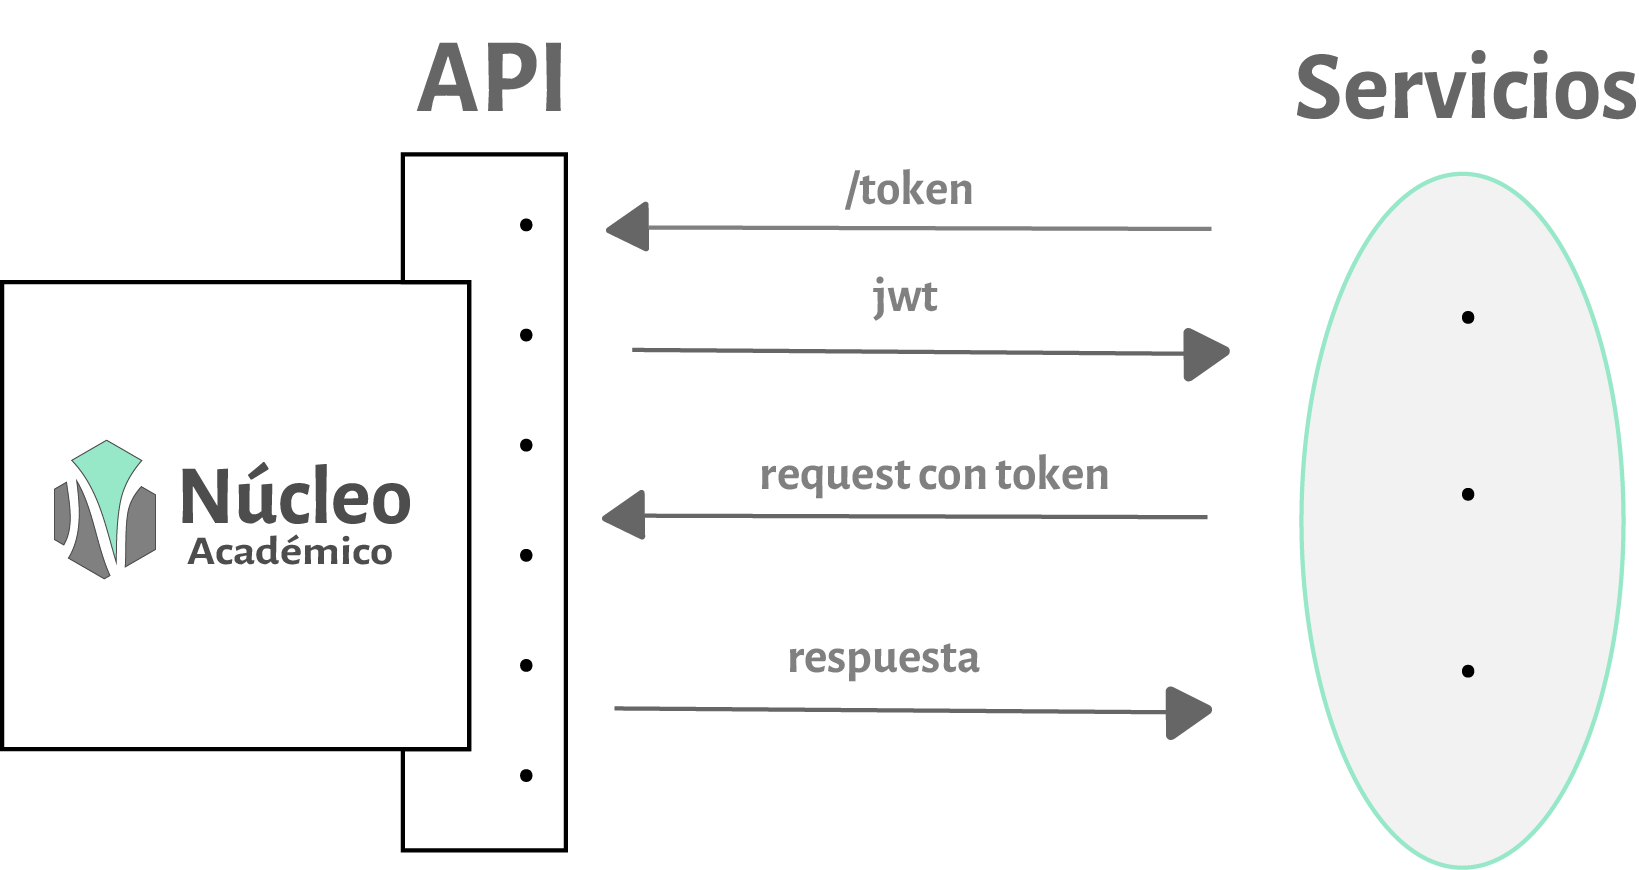
\includegraphics[scale=0.8]{images/nucleo/jwt.png}
  \captionof{figure}{Funcionamiento del pedido de token y posteriores requests}
  \label{fig:nucleo-jwt}
\end{figure}


\subsection{Deploy}

Para desplegar el núcleo se usa la siguiente configuración de docker-compose. Adicionalmente, se probaron configuraciones donde se disponen de varias instancias del núcleo limitando la cantidad de CPU y memoria de la que dispone cada uno. 

Esta es la configuración para una sola instancia, sin límite de CPU ni memoria.


\begin{minted}[gobble=4,frame=single,linenos]{yaml}
    
    # Se usa el formato 2.3 de docker-compose
    version: '2.3'
    # Defino los servicios a utilizar
    services:
      # En este caso, se muestra con una sola instancia
      nucleo-academico_1:
        # Defino el nombre del contenedor
        container_name: nucleo-academico_1
        # Siempre debe reiniciarse
        restart: always
        # El contexto de build es el directorio actual
        build: .
        # Defino el comando para iniciar la aplicación
        command: gunicorn -w 1 -b :8001 alumnos.wsgi:application
        # Defino los volúmenes
        volumes:
          - .:/code
        # Esta instancia va a estar corriendo en el puerto 8001
        ports:
          - "8001:8001"
        # Defino el archivo de configuraciones del entorno
        env_file:
          - ./.env
      # Pongo a nginx como otro servicio
      nginx:
        # Seteo el nombre del contenedor
        container_name: nginx-container
        restart: always
        build: ./nginx
        # Nginx va a correr en el puerto 8000 dentro del contenedor 
        # y hago un mapeo al 80 local
        ports:
          - "8000:80"
        # Le informo que va a depender del nucleo-academico_1
        depends_on:
          - nucleo-academico_1
    
    # Defino las networks, que serviran para conectar los contenedores
    networks:
      default:
        external:
          name: seguimiento-academico
  \end{minted}

\section[Análisis de Datos]{Análisis de Datos}

Para poder obtener información relevante de las carreras, materias y estudiantes, se debe hacer un análisis de los datos recopilados históricamente.

Si bien el núcleo provee una gran cantidad de datos, éstos necesitan una manipulación, procesamiento y una limpieza para que puedan ser analizados.

El objetivo principal de este módulo es de la obtención de los datos mediante una API Rest, la manipulación y el procesamiento de esos datos. Una vez terminado este proceso, sirve los resultados mediante una API Rest, que es consumida por un tercero para su visualización.

\subsection{Especificaciones}

El módulo de análisis de datos está construido con Python 3.6. El análisis de los datos se hizo con Pandas y los resultados son servidos gracias a Flask a través de una API REST.


La figura ~\ref{fig:analisis-nucleo} muestra el rol de este módulo y su funcionamiento con respecto al núcleo

\begin{figure}[h!]
  \centering
    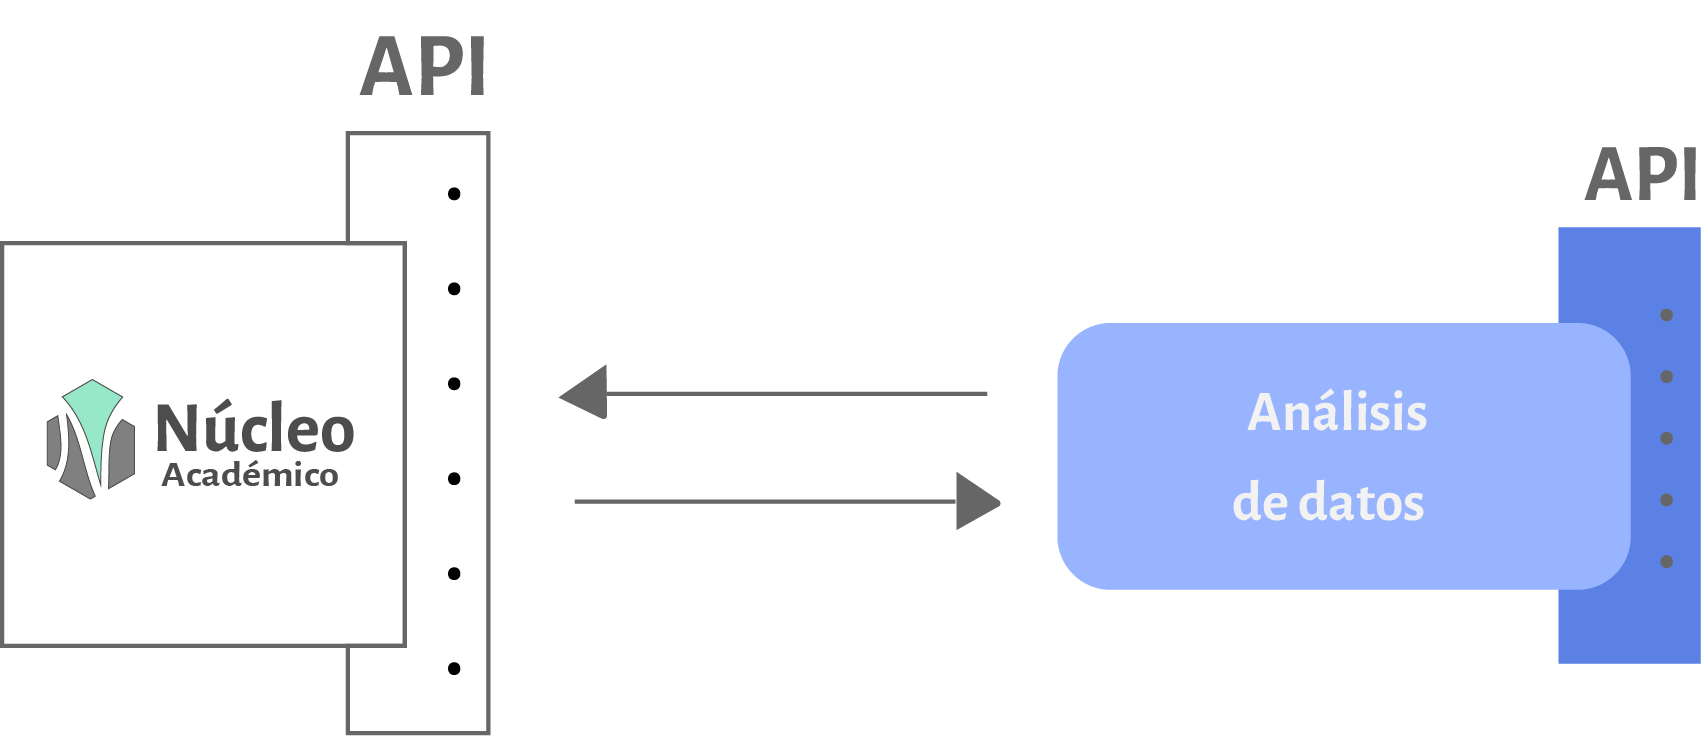
\includegraphics[scale=0.8]{images/analisis-datos/analisis-datos.png}
  \captionof{figure}{Obtención de datos a través del núcleo}
  \label{fig:analisis-nucleo}
\end{figure}

\subsection{Obtención de los datos}

Los datos son obtenidos a través de pedidos a la API del Núcleo. Estos datos llegan en forma de JSON y son transformados a DataFrame o Series (estructuras de datos de Pandas). 

Dado que los datos llegan de forma de recursos independientes, la mayor parte de los análisis requieren que estos datos sean unidos gracias a las funcionalidades de los DataFrames (de forma similar a los join de SQL).

\subsection{Análisis}

Una vez terminados los procesos de obtención, limpiado y union de los datos, se empieza el proceso de análisis.

Se realizaron análisis de diferentes magnitudes, basado en la cantidad de procesamiento que requieren. 
\subsubsection{Análisis sobre materias}

\paragraph{Datos basicos históricos} \mbox{}\\

URI: /materias/<cod\_materia>/basicos \\

Parámetros opcionales: inicio: yyyy-mm-dd, fin: yyyy-mm-dd, carrera: codigo de la carrera. \\

Dada una materia, analiza cuántos aprobaron, cuántos desaprobaron, cuántos quedaron ausentes y cuántos faltan aprobarla dentro de un período de tiempo.

\paragraph{Detalle de aprobación}\mbox{}\\

URI: /materias/<cod\_materia>/detalle-aprobados \\

Parámetros opcionales: inicio: yyyy-mm-dd, fin: yyyy-mm-dd, carrera: codigo de la carrera. \\

Dada una materia, dice el detalle de aprobados. Teniendo en cuenta la forma de aprobación. Las formas de aprobacion son:

>> Formas de aprobación

\paragraph{Dispersión de notas}\mbox{}\\

URI: /materias/<cod\_materia>/dispersion-notas \\

Parámetros opcionales: inicio: yyyy-mm-dd, fin: yyyy-mm-dd, carrera: codigo de la carrera. \\

Dada una materia, se hace un análisis de la dispersión de las notas dentro de un período. Teniendo en cuenta estudiantes, sus notas y el promedio de ese estudiante.

\paragraph{Número de recursantes}\mbox{}\\

URI: /materias/<cod\_materia>/recursantes \\

Parámetros opcionales: inicio: yyyy-mm-dd, fin: yyyy-mm-dd, carrera: codigo de la carrera. \\

Dada una materia, analiza qué estudiantes son recursantes y cuantas veces.


\subsubsection{Análisis sobre estudiantes}

\paragraph{Porcentaje de aprobación por área}\mbox{}\\

URI: /alumnos/<legajo>/porcentajes-areas \\

Parámetros adicionales: carrera, inicio, fin, plan \\

Dado un estudiante, se hace un análisis de los porcentajes de aprobación que tiene con respecto a las diferentes áreas de la carrera y el plan que se está analizando, dentro del período elegido.

Cada carrera tiene sus propias áreas. En particular, y tomado a forma de ejemplo, las áreas de la Licenciatura en Informática se muestran en la tabla ~\ref{tab:tabla_areas}.

\begin{table}[!htbp]
    \centering
    \makegapedcells
    \begin{tabular}{|c|c|}
    \hline
    Nombre \\ \hline
    Programación \\ \hline
    Sistemas Informáticos \\ \hline
    Procesos Informáticos\\ \hline
    Desarrollo de Software \\ \hline
    Teoría de la Computación \\ \hline
    \end{tabular}
    \caption{Áreas de la Licenciatura en Informática}
    \label{tab:tabla_areas}
\end{table}

\paragraph{Porcentaje de aprobación por núcleo}\mbox{}\\

URI: /alumnos/<legajo>/porcentajes-nucleos \\

Parámetros adicionales: carrera, inicio, fin, plan \\

Dado un estudiante, se hace un análisis de los porcentajes de aprobación que tiene con respecto a los diferentes núcleos de la carrera y el plan que se está analizando, dentro del período elegido.

Cada carrera tiene sus propias núcleos. En particular, y tomado a forma de ejemplo, los núcleos de la Licenciatura en Informática se muestran en la tabla ~\ref{tab:tabla_nucleos}.

\begin{table}[!htbp]
    \centering
    \makegapedcells
    \begin{tabular}{|c|c|}
    \hline
    Código & Nombre \\ \hline
    I & Introductorio \\ \hline
    B & Básico\\ \hline
    A & Avanzado \\ \hline
    C & Complementario/Orientativo \\ \hline
    \end{tabular}
    \caption{Núcleos de la Licenciatura en Informática}
    \label{tab:tabla_nucleos}
\end{table}


\paragraph{Notas}\mbox{}\\

URI: /alumnos/<legajo>/notas \\

Parámetros adicionales: carrera, inicio, fin, plan \\

Dado un estudiante, se obtienen las diferentes notas que tuvo a lo largo de sus cursadas.

\paragraph{Porcentaje de avance de carrera}\mbox{}\\

URI: /alumnos/<legajo>/porcentaje-carrera \\

Parámetros adicionales: carrera, inicio, fin, plan \\

Dado un legajo de estudiante, se realiza un análisis para determinar el porcentaje de avance de la carrera, según el plan que se analice. Dado que cada plan tiene una cantidad distinta de materias, este dato cambia según el plan que se analice.

\paragraph{Promedio por períodos}\mbox{}\\

URI: /alumnos/<legajo>/scores \\

Parámetros adicionales: carrera, inicio, fin, plan \\

Dado un estudiante, se calcula cuál fue su \textit{score} por cada período. Es decir, su rendimiento semestral. 

El \textit{score} se calcula sacando un promedio de sus notas en un semestre. Las materias que sólo se distinguen entre “Aprobado” y “Desaprobado” y no disponen de una nota, se les asigna una nota para sacar este promedio.
Las materias con nota “Aprobado” son consideradas como un 7, y las materias con nota “Desaprobado” son consideradas como un 3.

Entonces, el \textit{score} no es un promedio preciso, sino una estipulación de lo que fué su rendimiento en ese período.

Este score es útil para analizar el rendimiento de un estudiante y puede servirle a las carreras para tomar decisiones tempranas.

\subsubsection{Análisis sobre carreras}

\paragraph{Cantidad de estudiantes por semestre}\mbox{}\\

URI: /carreras/<carrera>/alumnos \\

Dada una carrera, se obtiene un listado de cantidad de inscriptos por semestre


\paragraph{Datos generales por cohorte}\mbox{}\\

URI: /carreras/<carrera>/cantidades-alumnos \\

Dada una carrera, se obtiene un listado de inscriptos, cursantes, graduados y postulantes por cohorte.


\paragraph{Ingresantes por cohorte}\mbox{}\\

URI: /carreras/<carrera>/cantidades-ingresantes \\

Dada una carrera, se obtiene la cantidad de ingresantes separadas por año.


\paragraph{Cantidad de cursantes actual}\mbox{}\\

URI: /carreras/<carrera>/cursantes-actual \\

Dada una carrera, se obtiene la cantidad de cursantes actual.


\paragraph{Cantidad de ingresantes actual}\mbox{}\\

URI: /carreras/<carrera>/ingresantes-actual \\

Dada una carrera, se obtiene la cantidad de ingresantes.


\paragraph{Cantidad total de graduados} \mbox{}\\

URI: /carreras/<carrera>/graduados-total \\

Dada una carrera, se obtiene el total de graduados.


\paragraph{Dispersión de scores y promedios}\mbox{}\\
URI: /carreras/<carrera>/dispersion-score-promedio \\

El objetivo de este análisis es el agrupar estudiantes en base al \textit{score} y al promedio. Mostrando grupos de interés sobre los cuales se podrán implementar acciones específicas.

\paragraph{Materias Traba}\mbox{}\\

URI: /carreras/<carrera>/materias-traba \\

Dada una carrera, se quiere analizar qué materias son las que traban a los estudiantes. 
Para poder realizar este análisis, se necesitaron los siguientes datos:
\begin{outline}
\1 Índice de aprobación de una materia (cantidad de aprobados / cantidad total de cursantes).
\1 Cuántas materias obligatorias dependen de ella.
\end{outline}

Luego de calcular estos datos materia por materia, se calcula un score. Este score determina qué materia puede llegar a trabar la carrera de un estudiante.

\begin{align*}
  Score = (1 - IndiceAprobacion) * CantidadObligatoriasDependientes\\
\end{align*}

Es decir, que una materia que tiene un porcentaje de aprobación del 75\% y 10 materias que son obligatorias y dependen de ésta para ser cursadas, tendrá un score de 2.5 ((1 - 0.75) * 10).



\section[Visualización de los datos analizados]{Visualización de los datos analizados}

Si bien la parte de análisis de datos quedó cubierta, se necesitó una forma de visualizarlos de forma gráfica. Por esta razón surgió la necesidad de crear una nueva aplicación independiente del núcleo y del análisis de datos.

Esta nueva aplicación obtuvo el nombre de Seguimiento Académico, y su logo se muestra en la figura ~\ref{fig:seguimiento-academico-logo}.

\begin{figure}[h!]
  \centering
    
\includegraphics[scale=0.5]{images/seguimiento-academico/seguimiento-academico-blanco.png}
  \captionof{figure}{Logo de la aplicación de Seguimiento Académico}
  \label{fig:seguimiento-academico-logo}
\end{figure}

Su objetivo principal es recolectar los datos analizados y mostrarlos de forma gráfica, dependiendo de los permisos que tenga el usuario que realiza el pedido.
Estos datos se desprenden del módulo de análisis, y se agrupan de la siguiente manera:

\begin{outline}
\2 Datos sobre carreras.
\2 Datos sobre materias.
\2 Datos sobre estudiantes.
\end{outline}

Cada uno de estos grupos de datos tiene su propia pantalla de tipo reporte, donde el usuario ingresa los parámetros necesarios para cada reporte.


\subsection{Especificaciones}

Seguimiento Académico esta construido con React 16.8 y se usó la libreria recharts para generar gráficos. Además, se uso el framework Material UI para el renderizado de elementos de la interfáz de usuario y diferentes tablas.
Este módulo realiza pedidos a la aplicación de análisis de datos, los cuales tienen que tener su correspondiente token para ser aceptados.
Cuando un usuario ingresa, se hace una autenticación con el núcleo. Esta autenticación tiene como resultado un token, y éste será utilizado para realizar todos los pedidos de datos correspondientes.

El gráfico ~\ref{fig:analisis-datos} muestra el rol de este módulo y su funcionamiento con respecto al de análisis de datos y al núcleo.

\begin{figure}[H]
  \centering
    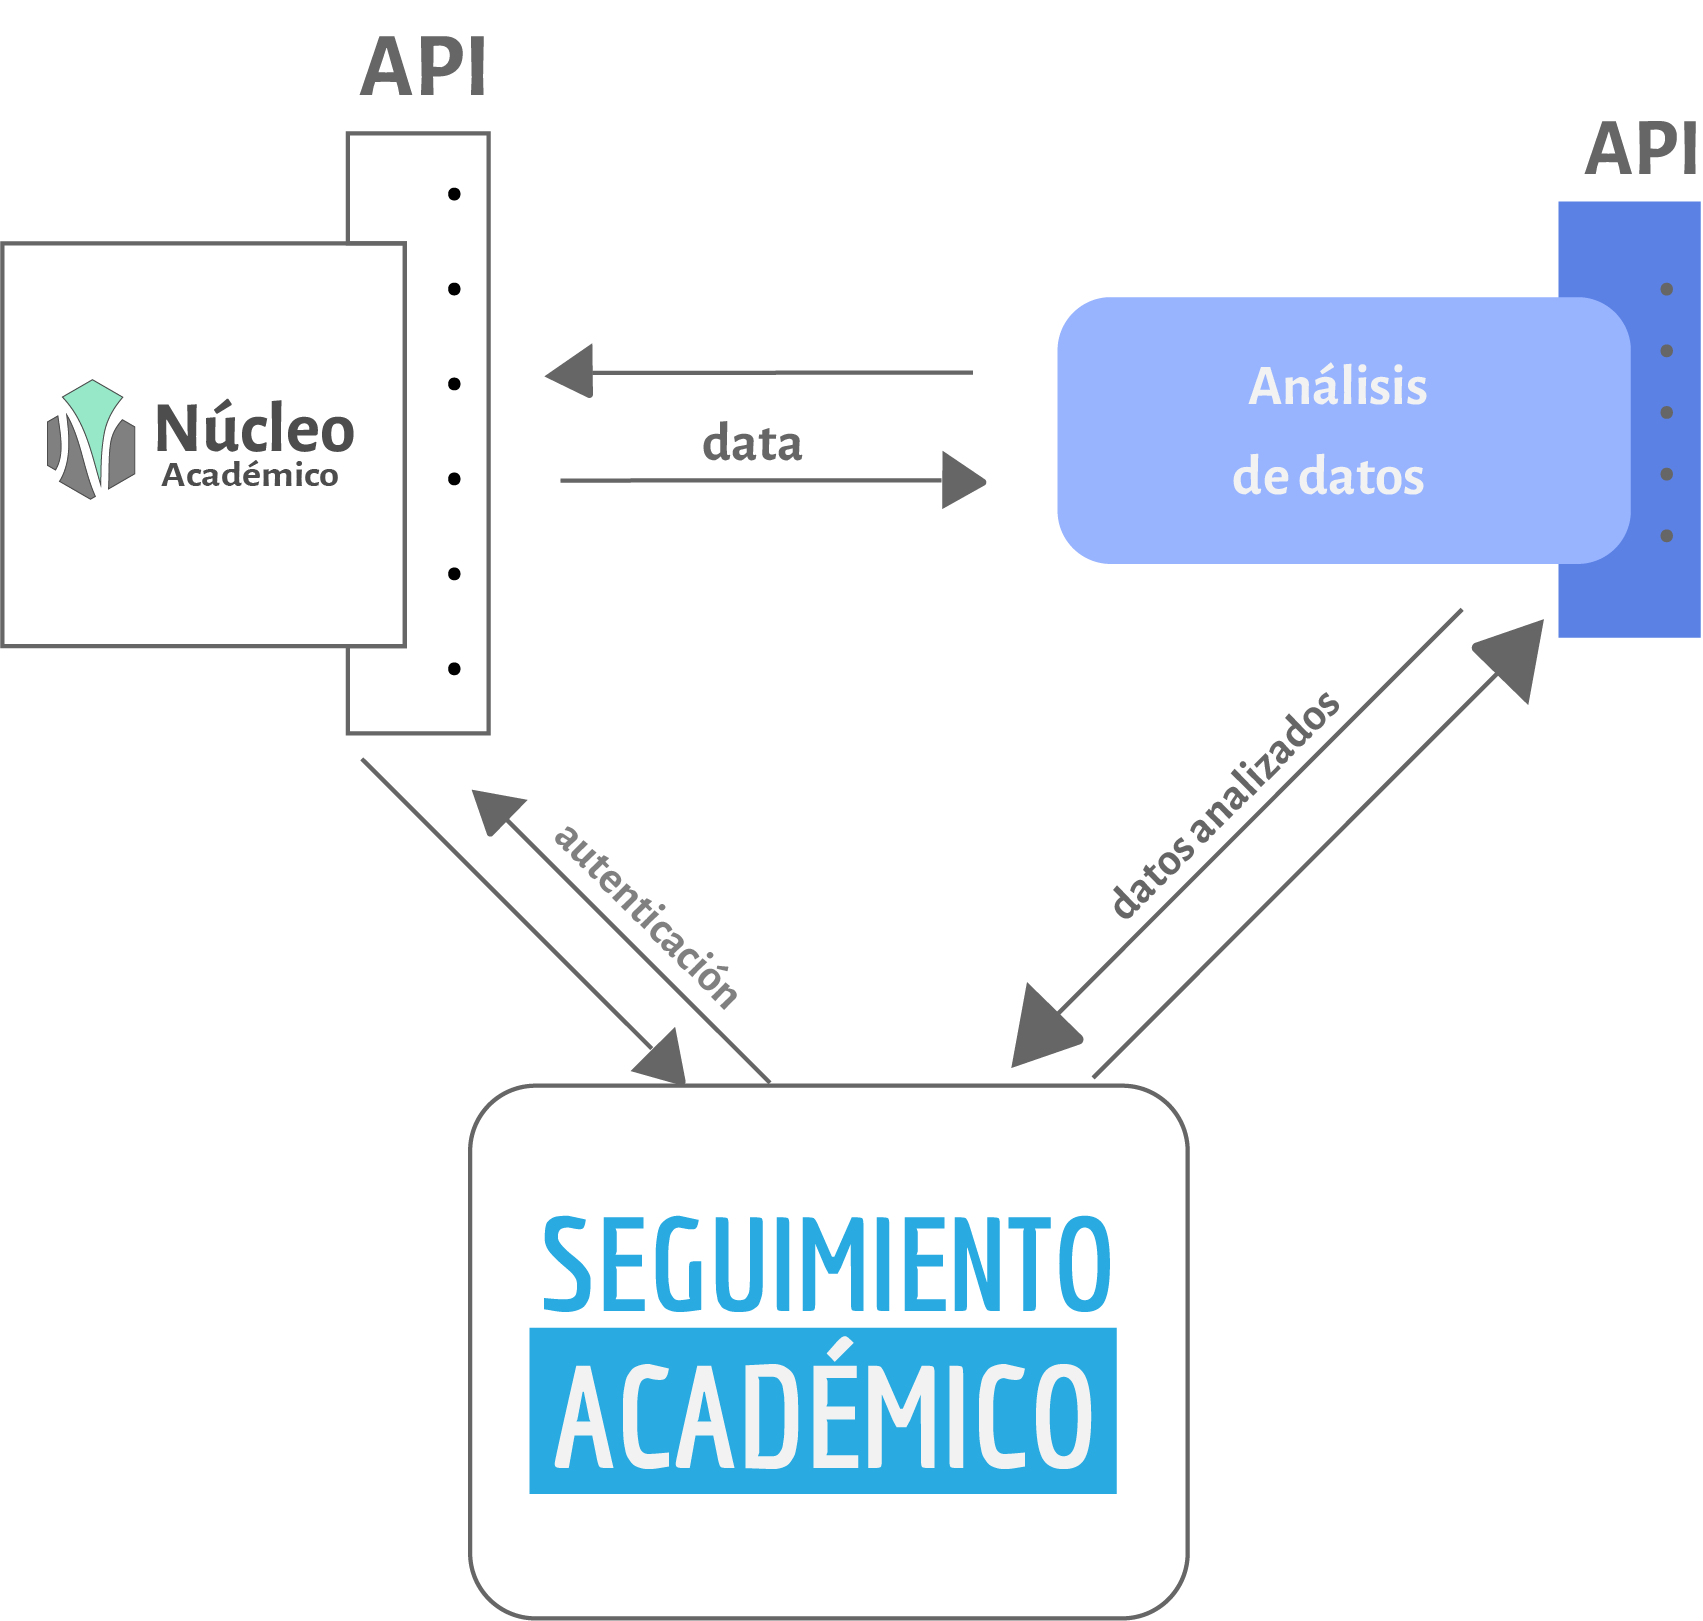
\includegraphics[scale=0.8]{images/seguimiento-academico/flow-seguimiento-academico.png}
  \captionof{figure}{Obtención de datos a través del núcleo}
  \label{fig:analisis-datos}
\end{figure}

\subsection{Obtención de los datos}

Los datos son obtenidos a través de pedidos a la API del módulo de análisis de datos gracias a Axios.
Axios está basado en \textit{promises}, con lo cual se puede aprovechar las ventajas de \textit{async} y \textit{await} para un código asincrónico más legible.

Estos pedidos se realizan a través de llamadas \textit{ajax}, lo cual quiere decir que la página carga normalmente y realiza los pedidos de forma asincrónica e independiente entre los gráficos. A medida que los datos van llegando, cada gráfico se va \textit{renderizando}.

Estos datos llegan como JSON y son procesados para ser mostrados de forma correcta.


\subsection{Visualización de datos}

La aplicación Seguimiento Académico tiene 5 pantallas principales:
\begin{outline}
 \1 Login (figura ~\ref{fig:sa-login}).
 \1 Home (figura ~\ref{fig:sa-home})
 \1 Reporte de Carrera (figura ~\ref{fig:sa-carrera})
 \1 Reporte de Materia (figura ~\ref{fig:sa-materia})
 \1 Reporte de Alumno (figura ~\ref{fig:sa-alumno})
\end{outline}

\subsubsection{Visualización por carrera}

Se dispone de un formulario para realizar un reporte, donde el usuario puede seleccionar entre sus carreras disponibles. Una vez que el formulario fue completado, se muestran los siguientes gráficos.

\paragraph{Cantidad actual de cursantes} \mbox{}\\
La cantidad actual de cursantes de la carrera se muestra en forma de tarjeta informativa (figura~\ref{fig:sa-cursantes}). 

\begin{figure}[H]
  \centering
    
\includegraphics[scale=0.4]{images/seguimiento-academico/sa-cursantes.png}
  \captionof{figure}{Cantidad de cursantes}
  \label{fig:sa-cursantes}
\end{figure}

\paragraph{Cantidad actual de ingresantes} \mbox{}\\
La cantidad actual de ingresantes de la carrera se muestra en forma de tarjeta informativa (figura~\ref{fig:sa-ingresantes}).

\begin{figure}[H]
  \centering
    
\includegraphics[scale=0.4]{images/seguimiento-academico/sa-ingresantes.png}
  \captionof{figure}{Cantidad de ingresantes}
  \label{fig:sa-ingresantes}
\end{figure}

\paragraph{Cantidad total de graduados} \mbox{}\\
La cantidad total de graduados de la carrera se muestra en forma de tarjeta informativa (figura~\ref{fig:sa-graduados}).

\begin{figure}[H]
  \centering
    
\includegraphics[scale=0.4]{images/seguimiento-academico/sa-graduados.png}
  \captionof{figure}{Cantidad de graduados}
  \label{fig:sa-graduados}
\end{figure}

\paragraph{Dispersión de estudiantes} \mbox{}\\
El siguiente gráfico muestra la dispersión de los estudiantes con respecto a su promedio general y su desempeño el último año. Uno de los ejes tiene en cuenta el promedio y el otro su score el último año. De esta manera, se puede observar de forma gráfica los estudiantes que se desempeñaron por encima de su historial y cuáles no (figura~\ref{fig:sa-dispersion}).

\begin{figure}[H]
  \centering
    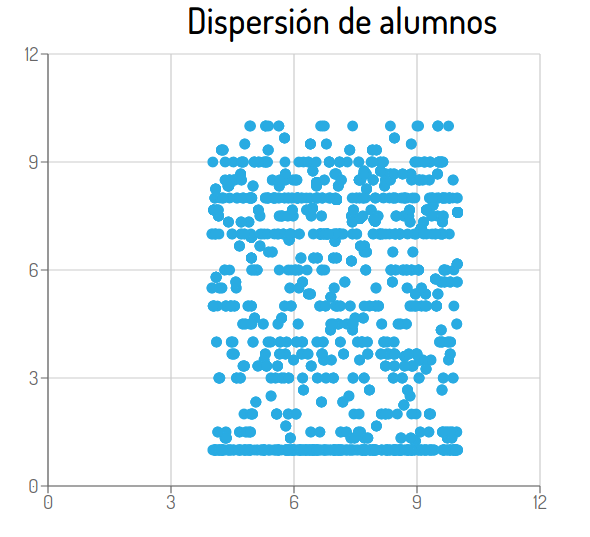
\includegraphics[scale=0.4]{images/seguimiento-academico/sa-dispersion.png}
  \captionof{figure}{Gráfico de dispersión}
  \label{fig:sa-dispersion}
\end{figure}

\paragraph{Cantidad de ingresos por semestre} \mbox{}\\
El siguiente gráfico es en forma de \textit{área}, y muestra la cantidad de ingresos semestrales histórico de la carrera. De esta forma, se puede observar en qué momento hubo picos de ingresos y en qué momentos hubo menos (figura~\ref{fig:sa-ingresos-semestre}).

\begin{figure}[H]
  \centering
    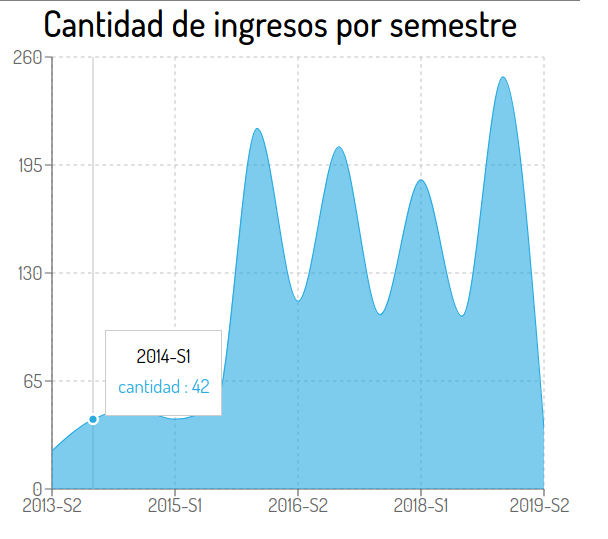
\includegraphics[scale=0.4]{images/seguimiento-academico/sa-ingresossemestre.png}
  \captionof{figure}{Ingresos por semestre}
  \label{fig:sa-ingresos-semestre}
\end{figure}

\paragraph{Alumnos por cohorte} \mbox{}\\
La siguiente es una tabla que detalla año a año de la carrera, qué cantidad de cursantes hubo, la cantidad de ingresantes y la cantidad de graduados  (figura~\ref{fig:sa-alumnos-cohorte}).

\begin{figure}[H]
  \centering
    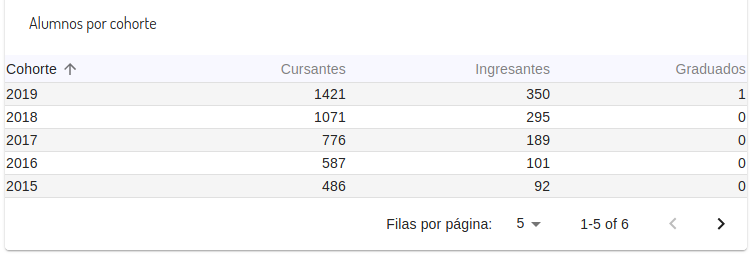
\includegraphics[scale=0.4]{images/seguimiento-academico/sa-alumnos-cohorte.png}
  \captionof{figure}{Tabla de alumnos por cohorte}
  \label{fig:sa-alumnos-cohorte}
\end{figure}

\paragraph{Ingresantes por cohorte} \mbox{}\\
La siguiente es una tabla que detalla año a año de la carrera, qué cantidad de ingresantes hubo  (figura~\ref{fig:sa-ingresantes-cohorte}).

\begin{figure}[H]
  \centering
    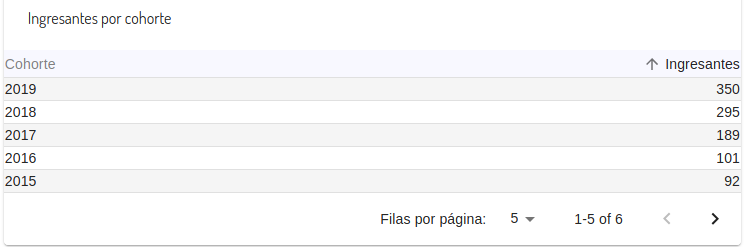
\includegraphics[scale=0.4]{images/seguimiento-academico/sa-ingresantes-cohorte.png}
  \captionof{figure}{Tabla de ingresantes por cohorte}
  \label{fig:sa-ingresantes-cohorte}
\end{figure}

\paragraph{Materias traba} \mbox{}\\
La siguiente tabla muestra un puntaje por materia en base a su porcentaje de aprobación y sobre la dependencia que tienen otras materias sobre ésta para ser cursadas  (figura~\ref{fig:sa-materias-traba}).

\begin{figure}[H]
  \centering
    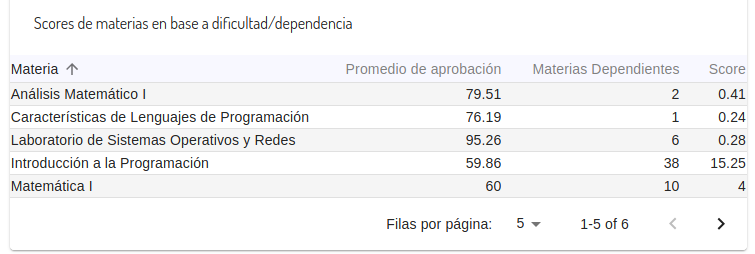
\includegraphics[scale=0.4]{images/seguimiento-academico/sa-materias-traba.png}
  \captionof{figure}{Tabla de ingresantes por cohorte}
  \label{fig:sa-materias-traba}
\end{figure}


\subsubsection{Visualización por materia}

Se dispone de un formulario para realizar un reporte, donde el usuario puede seleccionar entre sus carreras disponibles, luego ingresa el código de materia a analizar y una fecha de inicio y fin. De esta forma se analizará solo en el rango de fechas que se eligió.

Una vez que el formulario fue completado, se muestran los siguientes gráficos.

\paragraph{Estadísticas básicas de materia} \mbox{}\\
El siguiente gráfico muestra en forma de columnas los resultados de los estudiantes en el rango seleccionado. Se puede observar la cantidad de aprobados, ausentes, desaprobados y cuántos faltan cursarla  (figura~\ref{fig:sa-datos-basico}).

\begin{figure}[H]
  \centering
    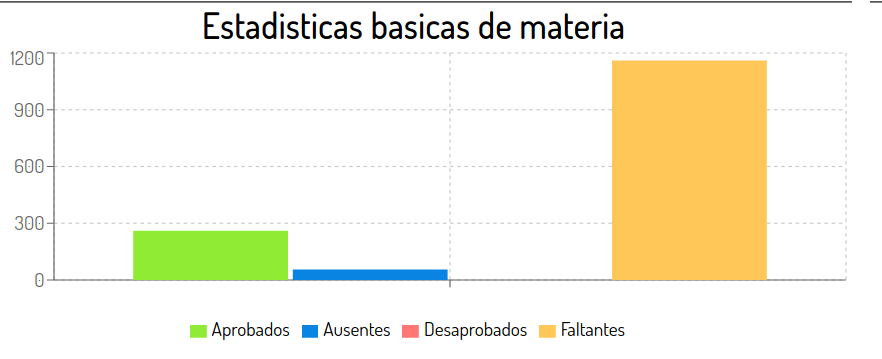
\includegraphics[scale=0.4]{images/seguimiento-academico/sa-datosbasicos.png}
  \captionof{figure}{Estadísticas básicas de la materia}
  \label{fig:sa-datos-basico}
\end{figure}

\paragraph{Detalle de aprobación} \mbox{}\\
El siguiente gráfico muestra en forma de columnas de qué forma aprobaron los estudiantes esa materia en el rango seleccionado. Se puede observar cuántos promocionaron en otra carrera, cuántos promocionaron, cuántos aprobaron un exámen equivalente, cuántos con una equivalencia equivalente y cuántos con exámen  (figura~\ref{fig:sa-detalle-aprobacion}).

\begin{figure}[H]
  \centering
    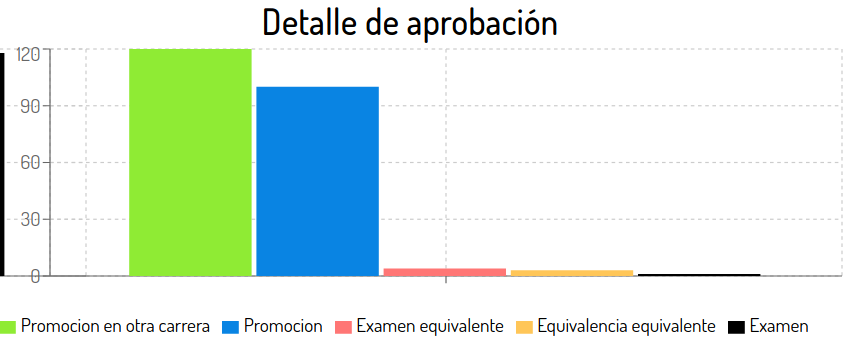
\includegraphics[scale=0.4]{images/seguimiento-academico/sa-detalleaprobacion.png}
  \captionof{figure}{Detalle de aprobación de la materia}
  \label{fig:sa-detalle-aprobacion}
\end{figure}

\paragraph{Dispersión de notas con respecto al promedio} \mbox{}\\
Este gráfico muestra en forma de dispersión como les fue a los estudiantes con respecto a su promedio.

\subsubsection{Visualización por alumno}
Se dispone de un formulario para realizar un reporte, donde el usuario puede seleccionar entre sus carreras disponibles, luego ingresa el legajo del estudiante a analizar, un plan de estudios, y una fecha de inicio y fin. De esta forma se analizará solo en el rango de fechas que se eligió.

Una vez que el formulario fue completado, se muestran los siguientes gráficos.

\paragraph{Desempeño del alumno} \mbox{}\\
El siguiente gráfico muestra el desempeño del alumno semestralmente dentro del rango seleccionado  (figura~\ref{fig:sa-detalle-aprobacion}).
\begin{figure}[H]
  \centering
    \includegraphics[scale=0.4]{images/seguimiento-academico/sa-desempeño.png}
  \captionof{figure}{Detalle de aprobación}
  \label{fig:sa-detalle-aprobacion}
\end{figure}

\paragraph{Porcentaje de carrera} \mbox{}\\
Se muestra el porcentaje de aprobación de la carrera en forma de tarjeta informativa.

\paragraph{Porcentajes de aprobación por área} \mbox{}\\
El siguiente gráfico de radar muestra los porcentajes de aprobación del alumno dentro de las áreas de la carrera (figura~\ref{fig:sa-porcentaje-area}).

\begin{figure}[H]
  \centering
    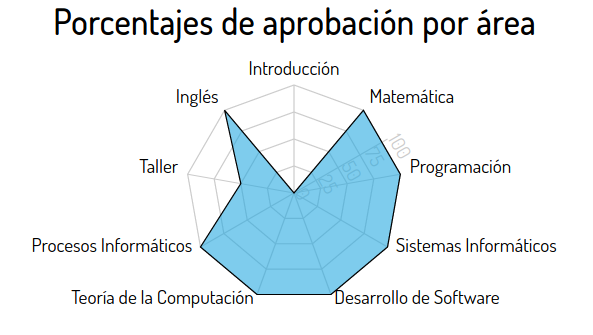
\includegraphics[scale=0.4]{images/seguimiento-academico/sa-porcentajesarea.png}
  \captionof{figure}{Porcentajes de aprobación por área}
  \label{fig:sa-porcentaje-area}
\end{figure}

\paragraph{Porcentajes de aprobacion por núcleo} \mbox{}\\
El siguiente gráfico de radar muestra los porcentajes de aprobación del alumno dentro de los núcleos de la carrera (figura~\ref{fig:sa-porcentaje-nucleo}).

\begin{figure}[H]
  \centering
    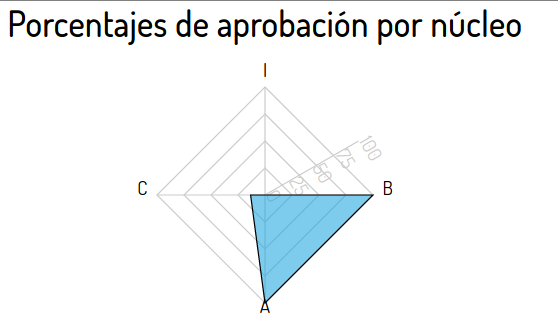
\includegraphics[scale=0.4]{images/seguimiento-academico/sa-porcentajesnucleo.png}
  \captionof{figure}{Porcentajes de aprobación por núcleo}
  \label{fig:sa-porcentaje-nucleo}
\end{figure}

\paragraph{Notas} \mbox{}\\
La siguiente tabla muestra las notas del alumno dentro del rango seleccionado (figura~\ref{fig:sa-notas}).

\begin{figure}[H]
  \centering
    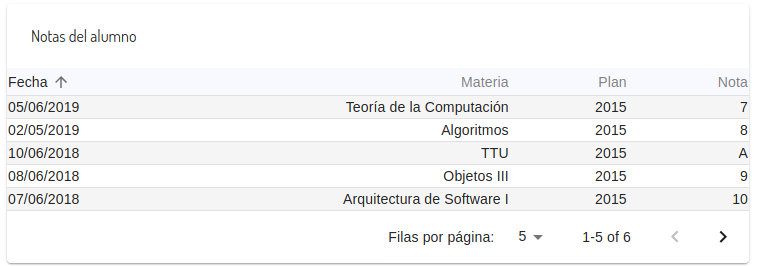
\includegraphics[scale=0.4]{images/seguimiento-academico/sa-notas.png}
  \captionof{figure}{Notas del alumno}
  \label{fig:sa-notas}
\end{figure}



\section{Licencia}
El código será licenciado bajo una licencia libre avalada por la OSI (Open Source Initiative) y la
FSF (Free Software Foundation). El código fuente será subido de forma pública a un repositorio
de código online de la UNQ para el libre acceso de todo aquel que desee utilizar, estudiar,
modificar, copia, redistribuir, mezclar, publicar o sublicenciar el software en cuestión.